\documentclass[a4paper,12pt]{scrartcl}


%------- Commands -----------------------------------------------------

\newcommand{\N}{\mathbb{N}}
\newcommand{\Z}{\mathbb{Z}}
\newcommand{\Q}{\mathbb{Q}}
\newcommand{\R}{\mathbb{R}}
\newcommand{\C}{\mathbb{C}}
\newcommand{\F}{\mathbb{F}}

\newcommand{\Aufg}{\stepcounter{Nummer}
	\textbf{Aufgabe \arabic{Nummer}:}}
\newcommand{\Lsg}{\textbf{L\"osungskommentar \arabic{Nummer}:}}
%------- Sprache --------------------------------------------------

% deutsche Silbentrennung
\usepackage[ngerman]{babel}
\let\latinencoding\relax



% eigene, zusätzliche Silbentrennung
\usepackage{hyphsubst} %Manuelle Sil\-ben\-tren\-nung



% Umlaute#
\usepackage[utf8]{inputenc}
 
  
  
\usepackage{amsmath}
\usepackage{amsfonts}
\usepackage{amssymb}
\usepackage{verbatim}  
  

%------- Formatierung --------------------------------------------------
  
% Seitenränder
\usepackage{geometry}
\geometry{a4paper, top= 25mm, bottom=20mm, left = 25mm, right = 25mm, footskip= 1cm}



% Querformat auf einzelner Seite \begin{landscape}

%\usepackage{lscape}


% Zeilenabstand (Unterscheidet sich evtl von den Standard 1.5)
%\usepackage{setspace}
%\linespread{1.5}


% no indent fürs Dokument.
\setlength\parindent{0pt}



% Seitenzahlen, hakt sich mit Kopfzeilen
% \pagestyle{plain}
% Späterer Beginn der Seitennummerierung: Kombinationen aus
%\thispagestyle{empty} und \setcounter{page}{1}



% Kopfzeilen



%Größen von Chapter usw ändern
%\makeatletter
%\renewcommand*{\size@chapter}{\Large}
%\renewcommand*{\size@section}{\large}
%\makeatother


%Kapitel ohne Nummer, aber im Inhaltsverzeichnis:
%\chapter*{Literaturverzeichnis}\addcontentsline{toc}{chapter}{Literaturverzeichnis}



%Fußnote \footnote{\label{foot:1}Korrekt gelesen!}

%------- Grafiken --------------------------------------------------

\usepackage{graphicx}
%\includegraphics[width=0.5\textwidth]{images/img1} oder scale=1





%------- Titelseite --------------------------------------------------

\begin{comment}

\begin{titlepage}
    \begin{center}
    \ \\ \vspace{30mm}
    \large \textbf{\textsf{Theoriebasierte Praxisreflexion}} \\
    \vspace{5mm}
    \LARGE\textbf{\textsf{Humor im Unterricht}}\\
    \vspace{1cm}
    \normalsize
    \today \\
    \vspace{9cm}
    \end{center}
 \normalsize{Tony Prange\\Boeselagerstraße 69a\\48163 Münster\\Matrikelnummer: 398873\\Email: tony.prange@wwu.de\\Abgabetermin 1. September 2016}
\end{titlepage}

\newpage  \tableofcontents \thispagestyle{empty} 

\end{comment}

% Zeilenabstand (Unterscheidet sich evtl von den Standard 1.5)
\usepackage{setspace}
\linespread{1.5}

\usepackage{fontspec}
%\setmainfont{Times New Roman}
\usepackage{booktabs}
\usepackage{multirow}
\usepackage{wrapfig}
%\usepackage{caption}

\usepackage{cancel}

\usepackage{colortbl}
\usepackage{xcolor}
%\usepackage{hyperref}
%\usepackage[all]{hypcap}
\usepackage{float}

%\usepackage{rotating}
%\newcommand\tabrotate[1]{\begin{turn}{45}\rlap{#1}\end{turn}}

\usepackage{pdfpages}
\usepackage[headsepline]{scrpage2}
\pagestyle{scrheadings}
\clearscrheadfoot

\ofoot{\pagemark}
\ohead{\normalfont \headmark}
\cfoot{\normalfont Mathematik \& Informatik}
\automark{section}
\newcommand{\gr}{\grqq{}}
\newcommand{\gl}{\glqq}
\newcommand{\vs}{\vspace{3pt}}
\newcommand{\red}{{ \color{red} Quelle}} 
\newcommand{\LL}{\ensuremath{\mathcal{L}}}

\renewcaptionname{ngerman}{\figurename}{\small{Abb.}}
\renewcaptionname{ngerman}{\tablename}{\small{Tab.}}
\newcommand{\Val}{Valenz und Herausforderung}
\newcommand{\norm}[1]{\left\| #1 \right\|}
\begin{document}
	
	
\begin{singlespace}
\begin{titlepage}
	\begin{center}
		
		
\includegraphics[scale=0.6]{wwu}
		
		\large{\textbf{\textsf{Institut für Bildungswissenschaften}}\\ 
			Sommersemester 2019} \\
		\vspace{20mm}
        \rule{.8\linewidth}{1pt}\\
        \vspace{3mm}
		\LARGE\textbf{\textsf{Umsetzung der Kouninschen Klassenführungsdimension \gl Valenz und Herausforderung\gr{} in meinem beruflichen Handeln}}\\
		%\rule{.2\linewidth}{.5pt}\\
		\rule{.8\linewidth}{1pt}\\

		\vfill
	\end{center}
\begin{flushright}
	\flushright

		\begin{large}
	\singlespacing 		
		\begin{tabular}{rl}

			eingereicht von: & \\
			 & Matrikelnr.: \\
			 & MEd für Gymnasien und Gesamtschulen\\
			 Fächerkombination: & Mathematik \& Informatik\\
			 \midrule
			Dozentin: & Dr. Kristina Antonette Frey   \\
			in:& Die weltberühmten  \\
			 & Klassenführungsdimensionen Jacob Kounins\\
			 & (066861)\\
			Leistungsart: & Prüfungsleistung\\
			Abgabefrist: & 01.09.2019

		\end{tabular}
		\end{large}	
\end{flushright}
	
\flushleft
\end{titlepage}

\newpage  \tableofcontents \thispagestyle{empty} \vspace{15mm}
\begin{center}
	\parbox{.8\linewidth}{\begin{small}
			{Beim Nachweis von Zitaten und Literatur wenden wie die von Unisa 
				vorgeschriebene Harvard-Methode an und folge dabei den Regeln 
				in: 
				
				Christof Sauer (Hg.) 2004. 
				Form bewahren: Handbuch zur 
				Harvard-Methode. 
				(GBFE-Studienbrief 5). Lage: Gesellschaft für 
				Bildung und Forschung in Europa e.V. 1. Auflage.} \\
			
			\end{small}}
\end{center}

\end{singlespace}
\newpage
\setcounter{page}{1}

\section*{Abstract}

\section{Introduction}
Durch die Vernetzung unserer digitalen Geräte, die unseren Alltag prägen und mitgestalten, ist eine große Menge an Daten vorhanden. Die Verwendung solcher Daten und der damit verbundenen Informationen ist ein Kernelement der heutigen Digitalgesellschaft. Programme, die solche Daten verwerten können, um möglichst viele Informationen zu generieren, spielen in unserer modernen Gesellschaft eine große Rolle. Dies ist nicht nur auf der Ebene von kontextbezogene Werbung von großem Interesse, sondern auch im zur Verbesserung unseres Medizinwesens und unserer Verhaltensweisen. Beispielsweise optimieren schon heute viele Personen unter Zuhilfenahme digitaler Fitnesstracker, etc. ihren persönlichen Lebensstil. Auch das Herstellen eines gesunden Schlafrhythmus ist durch die Erkennung von Schlafphasen möglich. 

Im Kontext des Gesundheitswesens ist diese Technologie besonders zentral, denn einerseits kann sie präventiv eingesetzt werden. Beispielsweise können Personen über ihre eigenen Gewohnheiten informiert und bezüglich ihrer Risiken sensibilisiert werden, was sie zu einem gesünderen Lebensstil bewegen kann, welcher wiederum von der Technologie unterstützt werden kann. Aus medizinischer Perspektive ermöglicht man eine Überprüfung darüber, wie und wie gesund eine Person lebt, um dadurch Krankheiten gezielter bekämpfen zu können. Hierfür ist es beispielsweise wichtig, aus verschiedensten Sensordaten Aktivitäten sicher ableiten zu können. 

Die hier vorliegende Ausarbeitung entstand im Rahmen eines Informatikpraktikums in der Vorlesung Mustererkennung, geleitet von Prof. Dr. Xiaoyi Jiang und Sören Klemm mit dem Thema Behavioral context recognition in-the-wild from mobile sensors. Ziel des Projektes war es, auf der Basis des Extrasensory Datensatzes Multi-Label-Klassifizierung durchzuführen. Im Wesentlichen sollten dabei gesammelten Sensordaten Aktivitäten zugeordnet werden, in einer Zusatzaufgabe sollten die Benutzer anhand ihrer Daten erkannt werden können. 

--------------------------

Die besondere Herausforderung des Projektes bestand darin, dass einerseits die Methodik nicht vorgegeben war und andererseits Multi-Label-Klassifizierung mit einem Datensatz ausgeführt werden sollte, der viele missing labels beinhaltete. 


\section{Vorstellung des Datensatzes}

Der ExtraSensory Datensatz wurde in den Jahren 2015 und 2016 von Yonatan Vaizman and Katherine Ellis unter Aufsicht von Professor Gert Lanckriet erhoben. Er basiert auf den Sensordaten von Smartphones und Smartwatches, welche von 60 Teilnehmern in minütigem Takt produziert wurden. Das Besondere dieser Werte besteht darin, dass sie von normalen Alltagsgegenständen erzeugt wurden, mehrere Sensoren parallel verwendet wurden und die Daten in einem natürlichen und nicht gestellten Kontext entstanden. Die Sensoren umfassten unter anderen ein accelerometer, gyroscope, location und audio und wurden von beinahe allen Personen in einem Großteil der Aufnahmen verwendet.

Die Zuordnung der Segmente zu Aktivitäten fand im Großteil durch die Benutzer selbst statt, sie besaßen dabei die Option auf vorgegebene Labels oder selbst erstellte für die Beschreibung zurückzugreifen. Im Endeffekt ergaben sich so 377,346 Datenpunkte, welche mit einem oder mehreren der finalen 51 Labels beschrieben wurden. Die Labels repräsentieren dabei Mannigfaltiges, wie etwa in class, singing, stairs (going up), stairs (going down) oder talking.

Das bedeutet, dass zu jedem Datenpunkt ein Labelvektor mit 51 Einträgen existiert. Jeder Eintrag kann die Werte yes oder no beinhalten, muss aber keinen Wert besitzen, wenn die bewertende Person keine Informationen bezüglich des korrespondierenden Labels angab (NaN). Die folgende Betrachtung der Datenpunkte zeigt, dass in jedem Datenpunkt viele Labels unbetrachtet blieben:

	\begin{figure}[h]
		\begin{center}
			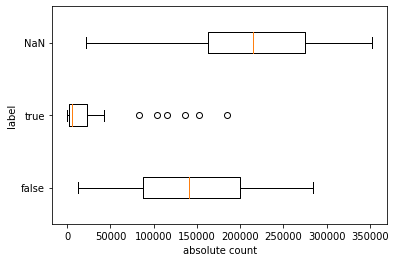
\includegraphics[scale=.8]{images/boxplot_label.png}
			\caption{XXXX}
			\label{abb:boxplot_label}
		\end{center}		
	\end{figure}	

Abbildung \ref{abb:boxplot_label} visualisiert die Verteilung der gesetzten Label-Werte als Box-Plot Diagramm. Zu erkennen ist, dass für die meisten Labels ein Großteil der Datenpunkte keinen Wert enthält - was die Klassifikation erschwert. Das heißt, es gibt für viele Labels eine große Anzahl von Datenpunkten, die erst einmal keine Information bezüglich des Labels beinhalten.

Weiter ist zu sehen, dass im Median zu jedem Label nur 5,153 yes-Eintragungen existieren und lediglich für sehr wenige Labels überhaupt mehr als 10\% der Datenpunkte eine yes-Eintragung.  Es gibt also viele Label-Klassen, die ausgesprochen wenig Repräsentanten beinhalten. 

\begin{figure}[h]
	\begin{center}
		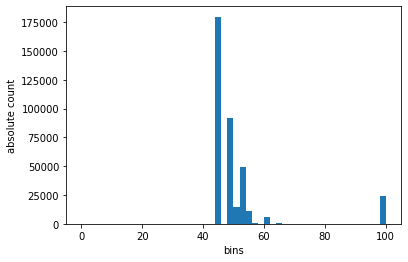
\includegraphics[scale=.8]{images/hist.png}
		\caption{XXXX}
		\label{abb:histogramm_data}
	\end{center}		
\end{figure}

Zuletzt ist zu erkennen, dass in allen Datenpunkten mindestens 44\% der 51 Labels nicht bewertet sind. Es gibt also keine Datenpunkte die zu allen Labels gleichzeitig Aussagen machen.


\subsection{Stand der Technik}


\section{Random Forests}

\subsection{Theorie}
\subsection{Praxis und Ergebnisse -> unzufrieden}

\section{Gradient Boosting}
\subsection{Theorie}

Der folgende Abschnitt orientiert sich an Chen, Guestrin (2016).

Beim Gradient Boosting geht es darum, iterativ eine Menge von gradient trees zu erzeugen, die ein gegebenes Klassifikationsproblem möglichst effektiv lösen.

Gradient trees sind im Wesentlichen decision trees, nur dass jedem Blatt des Baumes einen Wert, dessen Gewicht, $w_i$ zugewiesen wird. Folglich kann ein gradient tree mit $T$ Blättern und entsprechenden Gewichten $(w_1, .. ,w_T)$ als eine Funktion $f: \R^m \to \R$ aufgefasst werden. Jedem Datenpunkt $x \in \R^m$ wird unter $f$ das Gewicht des zu $x$ korrespondierenden Blattes zugeordnet $f(x) = w_{q(x)}$. $q: \R^m \to T$ ist dabei die Funktion, welche einem sample $x$ die Indexnummer des zu $x$ gehörigen Blattes zuweist. Weiter enthält $I_j := \{ i \mid q^{-1}(j)=x_i \}$ die Indizes derjenigen samples, welche auf das Blatt Nummer $j$ verweisen. Die Menge der gradient trees bezeichnen wir mit $\mathcal{F}$.

 Ein tree ensemble model $\{f_1, .. ,f_K \mid f_i \in \mathcal{F}\}$ bestehend aus $K$ gradient trees wird nicht, wie von decision trees bekannt, durch Voting ausgewertet, sondern indem die Funktionswerte des samples $x$ der einzelnen gradient trees in der ensemble Funktion $\Phi = \sum f_k$ aufsummiert werden. Das predicted outcome $\hat{y}$ eines samples $x$ ergibt sich damit zu:
 
 $$\hat{y} = \Phi(x) = \sum_{k=1}^{K} f_k(x)$$

Ist weiter eine Menge $X= \{(x_1), .. ,(x_n)\} \subset R^{m} $ von $n$ Beispielen mit jeweils $m$ features und dem zugehörigen ground truths $\{y_1, .. ,y_n\}$ gegeben, so erhält man die regularization funktion:

$$\mathcal{L} = \sum_{i=1}^{n} l(y_i, \Phi(x)) + \sum_{k=1}^{K}\Omega(f_k) \text{,  wobei } \Omega(f_k) = \gamma T + \frac{1}{2}\lambda \norm{w}_2^2$$

Bei $l$ handelt es sich um die loss-function, eine konvexe und mindestens mehrfach differenzierbare Funktion. $\Omega$ ist in diesem Kontext ein Strafterm und überwacht innerhalb von $\LL$ die Struktur des Baumes. Die Wahl von $\gamma$ beeinflusst die Anzahl der zulässigen Blätter, $\lambda$ die Gewichte ebendieser. Somit ist $\Omega$ eine Vorbeugemaßnahme gegen overfitting. Infolgedessen präferiert das mit $\LL$ erschaffene Modell gradient trees, die von einfacher Gestalt sind.


Das tatsächliche gradient tree boosting findet statt, indem iterativ neue Bäume dem Ensemble hinzugefügt werden. Im $t$-ten Iterationsschritt besteht das ensemble aus den in den vorigen Schritten erzeugten gradient trees $\{f_1, .. , f_{t-1}\}$. Ziel ist es, den neuen gradient tree $f_t$ so zu wählen, dass er das vorliegende model am meisten verbessert. Das ist genau dann der Fall, wenn
\begin{equation}
	\LL^{(t)} = \sum_{i=1}^{n} l(y_i, \Phi(x_i)) + \sum_{k=1}^{K}\Omega(f_k)
	\label{eq:LL1}
\end{equation}

minimal ist. Da die $\Omega(f_k)$ für die Bäume $f_1, .. , f_{t-1}$ bereits feststehen, spielen sie in der Betrachtung keine Rolle. Weiter stehen von $\Phi(x_i) = f_1(x_i) + .. + f_{t-1}(x_i) + f_t(x_i)$ bereits die ersten $t-1$ Summanden fest. Diese Summe wird in dem Ausdruck $\hat{y}^{t-1}$ zusammengefasst und ist konstant, da sie das predicted outcome nach dem $t-1$-ten Iterationsschritt des ensembles wiedergibt.

Damit lässt sich (\ref{eq:LL1}) auch formulieren als:
\begin{equation}
    \LL^{(t)} = \sum_{i=1}^{n} l(y_i, \hat{y}^{(t-1)} + f_k(x_i)) + \Omega(f_t)
    \label{eq:LL2}
\end{equation}

Um die Abhängigkeit von $l$ und $f_t$ zu trennen, wird die 1D-taylor series-expansion an der Stelle $(y_i,\hat{y}^{(t-1)})$ auf die Funktion $l$ und nur in der zweiten Koordinate ausgeführt. Obwohl es sich bei $l$ um eine 2D Funktion handelt, finden Änderungen im Kontext von $\LL$ nur in einer Koordinate statt, weshalb es berechtigt ist, sie als eine 1D-Funktion aufzufassen - etwa als $l(y_i,x) = l_{y_i}(x)$. Es ergibt sich:
\begin{equation}
\label{eq:taylor}
l_{y_i}(\hat{y}^{(t-1)} + f_k(x_i)) = l_{y_i}(\hat{y}^{(t-1)}) + l_{y_i}^{'}(\hat{y}^{(t-1)}) \cdot f_k(x_i)
+ \newline \frac{1}{2} l_{y_i}^{''}(\hat{y}^{(t-1)}) \cdot f_k(x_i)^2 + R_\text{taylor}
\end{equation}

Im Folgenden sei der Lesbarkeit halber $g_i = l_{y_i}^{'}(\hat{y}^{(t-1))}) ) = \frac{\partial l}{\partial \hat{y}^{(t-1)}}(y_i,\hat{y}^{(t-1)})$ und $h_i = l_{y_i}^{''}(\hat{y}^{(t-1)}) ) = \frac{\partial l}{\partial^2 \hat{y}^{(t-1)}}(y_i,\hat{y}^{(t-1)})$. Bei den $g_i$ und $h_i$ handelt es sich um Konstanten, denn sowohl $y_i$ als auch $\hat{y}^{(t-1))}$ sind im aktuellen Iterationsschritt bekannt. Wenden wir die Erkenntnisse aus Gleichung (\ref{eq:taylor}) auf $\LL^{(t)}$ an, ergibt sich somit:
\begin{equation}
	 \LL^{(t)} \approx \sum_{i=1}^{n} (l(y_i,\hat{y}^{(t-1)}) + g_if_t(x_i) + \frac{1}{2} h_i f_t(x_i)^2) + \Omega(f_t)
\end{equation}

Da die konstanten Terme $l(y_i,\hat{y}^{(t-1)})$ nicht von $f_t$ abhängen, können sie im Rahmen des Optimierungsproblems ignoriert werden und es ergibt sich das vereinfachte objective:
\begin{equation} \label{eq:LLeinfach}
\tilde{\LL}^{(t)} = \sum_{i=1}^{n}( g_if_t(x_i) + \frac{1}{2} h_i f_t(x_i)^2) + \Omega(f_t)
\end{equation}

Dieser Term kann jetzt vereinfacht werden, indem man $\Omega(f_t) = \gamma T + \frac{1}{2}\lambda \sum_{j=1}^{T} w_j^2$ ausschreibt. Für eine Baumstruktur $q$ ergeben sich die verschiedenen $I_j$, welche verwendet werden können, um die Summationsreihenfolge zu ändern. Dazu wird $f_t(x_i)$ als das korrespondierende Gewicht $w_j$ des neuen Baums $f_t$ ausgedrückt. Die Umsortierung erfolgt derart, dass nach den auftauchenden $w_j$ sortiert wird. Angewandt auf (\ref{eq:LLeinfach}) ergibt sich dann:
\begin{equation} \label{eq:LL_umsortiert}
	\tilde{\LL}^{(t)} = \sum_{j=1}^T\left( (\sum_{i \in I_j} g_i) w_j + \frac{1}{2} (\sum_{i \in I_j} h_i + \lambda)w_j^2 \right) + \gamma T
\end{equation}

Angemerkt werden muss, dass für diese Umsortierung und eine konkrete Auswertung des Terms der obigen Gleichung eine \textit{feste} Baumstruktur $q$ vorliegen muss. Das bedeutet, dass der Baum bis auf die Gewichte seiner Blätter bereits feststehen muss.

Um die optimierten Gewichte $w^*_j$ für diese feste Struktur von $f_t$ zu finden, leitet man $\tilde{\LL}^{(t)}$ aus Gleichung (\ref{eq:LL_umsortiert}) in Richtung des entsprechenden $w_j$ ab und erhält:
\begin{equation} \label{eq:LL_ableitung}
	\frac{\partial \tilde{\LL}^{(t)}}{\partial w_j} = \sum_{i \in I_j} g_i + (\sum_{i \in I_j} h_i + \lambda)w_j
\end{equation}

Setzt man diese Gleichung gleich $0$ und stellt sie um nach $w_j$, ergibt sich als das optimale $w^*_j$, welches $\tilde{\LL}^{(t)}$ minimiert:
\begin{equation}
	\label{eq:opt_w}
	w_j^* = - \frac{\sum_{i \in I_j} g_i}{\sum_{i \in I_j} h_i + \lambda}
\end{equation}

Unter Verwendung dieser optimalen $w_j^*$ ergibt sich eingesetzt in (\ref{eq:LL_umsortiert}) der Optimalwert von $\tilde{\LL}^{(t)}$ für die Baumstruktur $q$:

\begin{equation} \label{eq:entropy}
	\tilde{\LL}^{(t)} (q) = - \frac{1}{2} \sum_{j=1}^{T} \frac{(\sum_{i \in I_j} g_i)^2}{\sum_{i \in I_j} h_i + \lambda} + \gamma T
\end{equation}

Es ist also möglich, für eine gegebene Baumstruktur $q$ die für das ensemble besten Gewichte des neuen Baums $f_t$ zu berechnen. Weil es aber in der Realität nicht möglich ist, in jedem Iterationsschritt alle überhaupt möglichen Baumstrukturen zu bestimmen und bezüglich ihres Wertes $\tilde{\LL}^{(t)} (q)$ zu vergleichen, ..................................................

% Label hinzufügen:
% \label{eq:opt_w}
% \label{eq:entropy}

Es ist also möglich, für eine gegebene Baumstruktur $q$ die für das ensemble hilfreichsten Gewichte des neuen Baums $f_t$ unter Verwendung von (\ref{eq:opt_w}) zu berechnen. Weiter kann eine solche (optimierte) Baumstruktur $q$ mit (\ref{eq:entropy}) bewertet werden, diese Bewertung ist vergleichbar mit der Entropy von decision trees. 

In der Realität müsste man nun alle möglichen Baumstrukturen, inklusive der verschiedenen feature-splits, abarbeiten, die optimierten $w^*_j$ und $\tilde{\LL}^{(t)} (q)$ berechnen und vergleichen. Weil das aber kaum realisierbar ist, wird der Baum $f_t$ im Iterationsschritt $t$ greedy konstruiert. Dafür werden iterativ branches dem Baum hinzugefügt, die durch das Aufspalten eines Blattes entstehen. Sind $I_l, I_r$ die Mengen der dem linken beziehungsweise rechten Blatt zugewiesenen Indexnummern und $I = I_l \dot\cup I_r$ die Indexmenge des ehemaligen Blattes. Die resultierende Verbesserung dieses splits ergibt sich nach (\ref{eq:entropy}) zu:
\begin{equation}
\begin{split}
	\tilde{\LL}_\text{split} &= \tilde{\LL}^{(t)} (q_\text{alt})-\tilde{\LL}^{(t)} (q_\text{neu})\\
	&= \left( - \frac{1}{2} \sum_{j=1}^{T} \frac{(\sum\limits_{i \in I_{j, \text{alt}}} g_i)^2}{\sum\limits_{i \in I_{j, \text{neu}}} h_i + \lambda} + \gamma T \right)- \left( - \frac{1}{2} \sum_{j=1}^{T+1} \frac{(\sum\limits_{i \in I_{j, \text{neu}}} g_i)^2}{\sum\limits_{i \in I_{j, \text{neu}}} h_i + \lambda} + \gamma (T+1) \right)\\	
	&= \frac{1}{2} \left( \frac{(\sum_{i \in I_l} g_i)^2}{\sum_{i \in I_l} h_i + \lambda} + \frac{(\sum_{i \in I_r} g_i)^2}{\sum_{i \in I_r} h_i + \lambda} - \frac{(\sum_{i \in I} g_i)^2}{\sum_{i \in I} h_i + \lambda} \right) - \gamma 
\end{split}
\end{equation}

Die zweite Gleichheit folgt daraus, dass sich die Indexmengen $I_j$ bis auf des aufgeteilen Blattes, also die Indexmengen $I, I_l$ und $I_r$, nicht unterscheiden und somit aufheben. 

\subsection{Implementierungsdetails}
-> Multilabel einzeln trainieren

\subsection{eigene Variationen}
-> Hyperparametern
-> Geschwindigkeit (GPU)


\section{Vorstellung Results}
-> Metric

\section{Bewertung der Results}

\section{classification of users}

\section{Auswertung}
- Auswirkungen verschiedener Gewichte der Datenpunkte und sowas (Modifikationen an Input, etc)
- NaN Handling
- Findung der Parameter

\section{Fazit}

\newpage
\section{Literaturverzeichnis}

\hangindent+30pt \hangafter=1
\textsc{Drüke-Noe, C.} 2014. \textit{Aufgabenkultur in Klassenarbeiten im Fach Mathematik – Empirische Untersuchungen in neunten und zehnten Klassen}. Wiesbaden:
Springer Spektrum.









\newpage
\ohead{\normalfont Eigenständigkeitserklärung}
\addcontentsline{toc}{section}{Eigenständigkeitserklärung} 
\vspace*{1cm}
\begin{center}
	\Large \textbf{Anti-Plagiatserklärung}\\
	
	\large \textbf{Erklärung des Studierenden}
\end{center}

\normalsize
\vspace{25mm}
Hiermit versichere ich, dass ich die vorliegende Hausarbeit mit dem Namen \glqq {Umsetzung der Kouninschen Klassenführungsdimension \gl Valenz und Herausforderung\gr{} in meinem beruflichen Handeln\grqq{} selbstständig verfasst habe, und dass ich keine anderen Quellen und Hilfsmittel als die angegebenen benutzt habe und dass die Stellen der Arbeit, die anderen Werken – auch elektronischen Medien – dem Wortlaut oder Sinn nach entnommen wurden, auf jeden Fall unter Angabe der Quelle als Entlehnung kenntlich gemacht worden sind.\\
	
	
	
	
	\begin{center}
		\rule{6cm}{.5pt} \hspace{3cm} \rule{6cm}{.5pt}
	\end{center}	
	\vspace{-5mm}
	\hspace*{25mm} Ort, Datum	\hspace{70mm} Tony Prange


\end{document}